% Created by tikzDevice version 0.12 on 2019-03-20 11:38:21
% !TEX encoding = UTF-8 Unicode
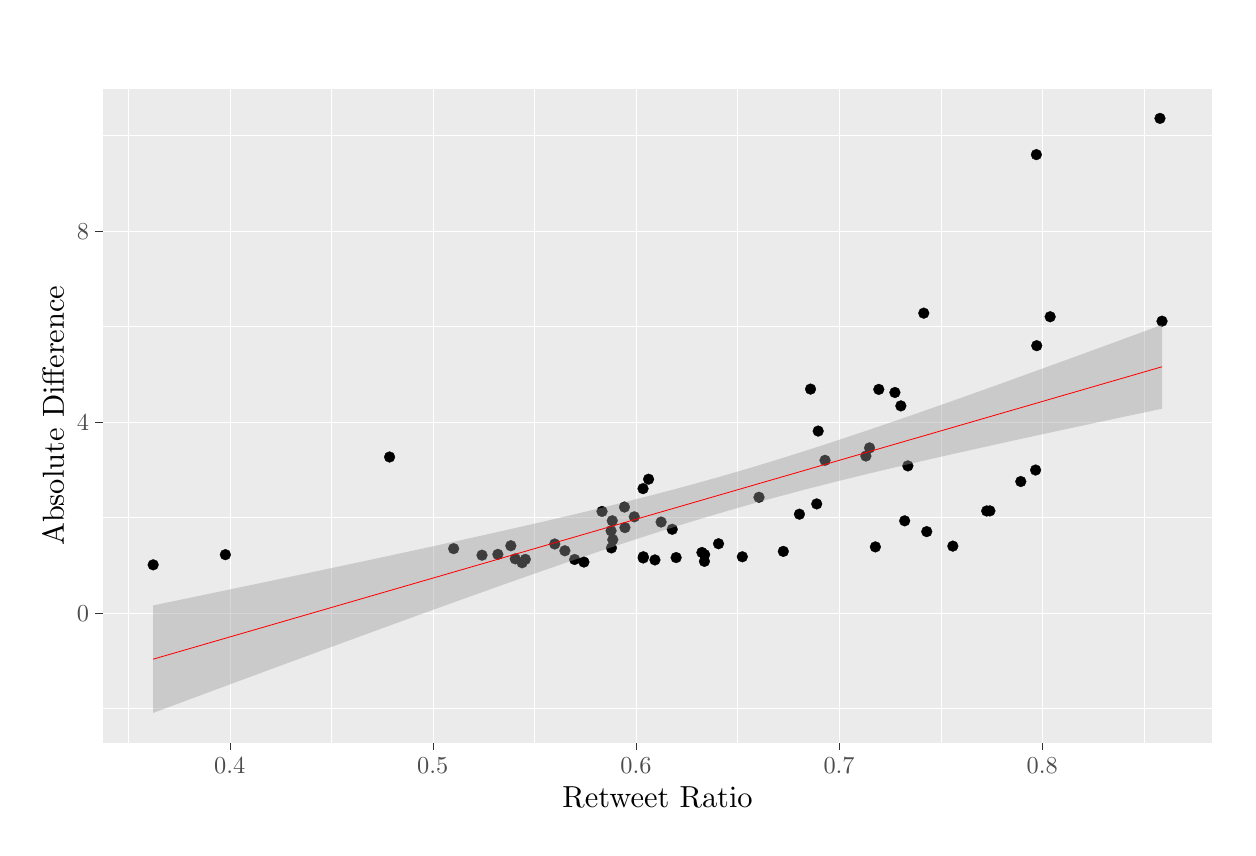
\begin{tikzpicture}[x=1pt,y=1pt]
\definecolor{fillColor}{RGB}{255,255,255}
\path[use as bounding box,fill=fillColor,fill opacity=0.00] (0,0) rectangle (433.62,289.08);
\begin{scope}
\path[clip] (  0.00,  0.00) rectangle (433.62,289.08);
\definecolor{drawColor}{RGB}{255,255,255}
\definecolor{fillColor}{RGB}{255,255,255}

\path[draw=drawColor,line width= 0.1pt,line join=round,line cap=round,fill=fillColor] (  0.00,  0.00) rectangle (433.62,289.08);
\end{scope}
\begin{scope}
\path[clip] ( 27.12, 30.73) rectangle (428.12,267.04);
\definecolor{fillColor}{gray}{0.92}

\path[fill=fillColor] ( 27.12, 30.73) rectangle (428.12,267.04);
\definecolor{drawColor}{RGB}{255,255,255}

\path[draw=drawColor,line width= 0.1pt,line join=round] ( 27.12, 43.13) --
	(428.12, 43.13);

\path[draw=drawColor,line width= 0.1pt,line join=round] ( 27.12,112.14) --
	(428.12,112.14);

\path[draw=drawColor,line width= 0.1pt,line join=round] ( 27.12,181.14) --
	(428.12,181.14);

\path[draw=drawColor,line width= 0.1pt,line join=round] ( 27.12,250.14) --
	(428.12,250.14);

\path[draw=drawColor,line width= 0.1pt,line join=round] ( 36.28, 30.73) --
	( 36.28,267.04);

\path[draw=drawColor,line width= 0.1pt,line join=round] (109.69, 30.73) --
	(109.69,267.04);

\path[draw=drawColor,line width= 0.1pt,line join=round] (183.10, 30.73) --
	(183.10,267.04);

\path[draw=drawColor,line width= 0.1pt,line join=round] (256.50, 30.73) --
	(256.50,267.04);

\path[draw=drawColor,line width= 0.1pt,line join=round] (329.91, 30.73) --
	(329.91,267.04);

\path[draw=drawColor,line width= 0.1pt,line join=round] (403.32, 30.73) --
	(403.32,267.04);

\path[draw=drawColor,line width= 0.1pt,line join=round] ( 27.12, 77.64) --
	(428.12, 77.64);

\path[draw=drawColor,line width= 0.1pt,line join=round] ( 27.12,146.64) --
	(428.12,146.64);

\path[draw=drawColor,line width= 0.1pt,line join=round] ( 27.12,215.64) --
	(428.12,215.64);

\path[draw=drawColor,line width= 0.1pt,line join=round] ( 72.99, 30.73) --
	( 72.99,267.04);

\path[draw=drawColor,line width= 0.1pt,line join=round] (146.39, 30.73) --
	(146.39,267.04);

\path[draw=drawColor,line width= 0.1pt,line join=round] (219.80, 30.73) --
	(219.80,267.04);

\path[draw=drawColor,line width= 0.1pt,line join=round] (293.21, 30.73) --
	(293.21,267.04);

\path[draw=drawColor,line width= 0.1pt,line join=round] (366.62, 30.73) --
	(366.62,267.04);
\definecolor{drawColor}{RGB}{0,0,0}
\definecolor{fillColor}{RGB}{0,0,0}

\path[draw=drawColor,line width= 0.1pt,line join=round,line cap=round,fill=fillColor] (232.91,107.82) circle (  1.96);

\path[draw=drawColor,line width= 0.1pt,line join=round,line cap=round,fill=fillColor] (194.12,100.06) circle (  1.96);

\path[draw=drawColor,line width= 0.1pt,line join=round,line cap=round,fill=fillColor] (243.64, 99.44) circle (  1.96);

\path[draw=drawColor,line width= 0.1pt,line join=round,line cap=round,fill=fillColor] (210.94,101.08) circle (  1.96);

\path[draw=drawColor,line width= 0.1pt,line join=round,line cap=round,fill=fillColor] (313.37,157.25) circle (  1.96);

\path[draw=drawColor,line width= 0.1pt,line join=round,line cap=round,fill=fillColor] (201.00, 95.98) circle (  1.96);

\path[draw=drawColor,line width= 0.1pt,line join=round,line cap=round,fill=fillColor] (210.81,107.27) circle (  1.96);

\path[draw=drawColor,line width= 0.1pt,line join=round,line cap=round,fill=fillColor] (264.26,119.39) circle (  1.96);

\path[draw=drawColor,line width= 0.1pt,line join=round,line cap=round,fill=fillColor] (273.05, 99.83) circle (  1.96);

\path[draw=drawColor,line width= 0.1pt,line join=round,line cap=round,fill=fillColor] (228.89,110.43) circle (  1.96);

\path[draw=drawColor,line width= 0.1pt,line join=round,line cap=round,fill=fillColor] (244.62, 98.67) circle (  1.96);

\path[draw=drawColor,line width= 0.1pt,line join=round,line cap=round,fill=fillColor] (249.64,102.60) circle (  1.96);

\path[draw=drawColor,line width= 0.1pt,line join=round,line cap=round,fill=fillColor] (211.43,104.06) circle (  1.96);

\path[draw=drawColor,line width= 0.1pt,line join=round,line cap=round,fill=fillColor] (364.21,129.23) circle (  1.96);

\path[draw=drawColor,line width= 0.1pt,line join=round,line cap=round,fill=fillColor] (153.92,100.83) circle (  1.96);

\path[draw=drawColor,line width= 0.1pt,line join=round,line cap=round,fill=fillColor] (190.46,102.51) circle (  1.96);

\path[draw=drawColor,line width= 0.1pt,line join=round,line cap=round,fill=fillColor] (409.15,256.30) circle (  1.96);

\path[draw=drawColor,line width= 0.1pt,line join=round,line cap=round,fill=fillColor] (258.24, 97.89) circle (  1.96);

\path[draw=drawColor,line width= 0.1pt,line join=round,line cap=round,fill=fillColor] (347.69,114.47) circle (  1.96);

\path[draw=drawColor,line width= 0.1pt,line join=round,line cap=round,fill=fillColor] (409.89,183.02) circle (  1.96);

\path[draw=drawColor,line width= 0.1pt,line join=round,line cap=round,fill=fillColor] (164.17, 98.46) circle (  1.96);

\path[draw=drawColor,line width= 0.1pt,line join=round,line cap=round,fill=fillColor] (174.59,101.87) circle (  1.96);

\path[draw=drawColor,line width= 0.1pt,line join=round,line cap=round,fill=fillColor] (224.36,125.92) circle (  1.96);

\path[draw=drawColor,line width= 0.1pt,line join=round,line cap=round,fill=fillColor] (226.66, 96.75) circle (  1.96);

\path[draw=drawColor,line width= 0.1pt,line join=round,line cap=round,fill=fillColor] (215.64,115.85) circle (  1.96);

\path[draw=drawColor,line width= 0.1pt,line join=round,line cap=round,fill=fillColor] (215.82,108.43) circle (  1.96);

\path[draw=drawColor,line width= 0.1pt,line join=round,line cap=round,fill=fillColor] (219.19,112.33) circle (  1.96);

\path[draw=drawColor,line width= 0.1pt,line join=round,line cap=round,fill=fillColor] (364.49,243.21) circle (  1.96);

\path[draw=drawColor,line width= 0.1pt,line join=round,line cap=round,fill=fillColor] (323.80,185.92) circle (  1.96);

\path[draw=drawColor,line width= 0.1pt,line join=round,line cap=round,fill=fillColor] (364.62,174.16) circle (  1.96);

\path[draw=drawColor,line width= 0.1pt,line join=round,line cap=round,fill=fillColor] (211.24,110.90) circle (  1.96);

\path[draw=drawColor,line width= 0.1pt,line join=round,line cap=round,fill=fillColor] ( 45.35, 94.98) circle (  1.96);

\path[draw=drawColor,line width= 0.1pt,line join=round,line cap=round,fill=fillColor] ( 71.44, 98.65) circle (  1.96);

\path[draw=drawColor,line width= 0.1pt,line join=round,line cap=round,fill=fillColor] (176.19, 97.14) circle (  1.96);

\path[draw=drawColor,line width= 0.1pt,line join=round,line cap=round,fill=fillColor] (346.54,114.44) circle (  1.96);

\path[draw=drawColor,line width= 0.1pt,line join=round,line cap=round,fill=fillColor] (315.52,152.41) circle (  1.96);

\path[draw=drawColor,line width= 0.1pt,line join=round,line cap=round,fill=fillColor] (178.67, 95.73) circle (  1.96);

\path[draw=drawColor,line width= 0.1pt,line join=round,line cap=round,fill=fillColor] (179.83, 96.95) circle (  1.96);

\path[draw=drawColor,line width= 0.1pt,line join=round,line cap=round,fill=fillColor] (169.90, 98.75) circle (  1.96);

\path[draw=drawColor,line width= 0.1pt,line join=round,line cap=round,fill=fillColor] (222.46, 97.90) circle (  1.96);

\path[draw=drawColor,line width= 0.1pt,line join=round,line cap=round,fill=fillColor] (130.77,133.94) circle (  1.96);

\path[draw=drawColor,line width= 0.1pt,line join=round,line cap=round,fill=fillColor] (306.32,101.46) circle (  1.96);

\path[draw=drawColor,line width= 0.1pt,line join=round,line cap=round,fill=fillColor] (324.87,106.98) circle (  1.96);

\path[draw=drawColor,line width= 0.1pt,line join=round,line cap=round,fill=fillColor] (222.42, 97.46) circle (  1.96);

\path[draw=drawColor,line width= 0.1pt,line join=round,line cap=round,fill=fillColor] (282.89,158.48) circle (  1.96);

\path[draw=drawColor,line width= 0.1pt,line join=round,line cap=round,fill=fillColor] (302.88,134.29) circle (  1.96);

\path[draw=drawColor,line width= 0.1pt,line join=round,line cap=round,fill=fillColor] (222.36,122.51) circle (  1.96);

\path[draw=drawColor,line width= 0.1pt,line join=round,line cap=round,fill=fillColor] (358.86,125.08) circle (  1.96);

\path[draw=drawColor,line width= 0.1pt,line join=round,line cap=round,fill=fillColor] (369.47,184.62) circle (  1.96);

\path[draw=drawColor,line width= 0.1pt,line join=round,line cap=round,fill=fillColor] (207.54,114.27) circle (  1.96);

\path[draw=drawColor,line width= 0.1pt,line join=round,line cap=round,fill=fillColor] (318.05,130.73) circle (  1.96);

\path[draw=drawColor,line width= 0.1pt,line join=round,line cap=round,fill=fillColor] (285.11,116.99) circle (  1.96);

\path[draw=drawColor,line width= 0.1pt,line join=round,line cap=round,fill=fillColor] (197.64, 96.91) circle (  1.96);

\path[draw=drawColor,line width= 0.1pt,line join=round,line cap=round,fill=fillColor] (234.32, 97.60) circle (  1.96);

\path[draw=drawColor,line width= 0.1pt,line join=round,line cap=round,fill=fillColor] (288.12,132.74) circle (  1.96);

\path[draw=drawColor,line width= 0.1pt,line join=round,line cap=round,fill=fillColor] (278.87,113.27) circle (  1.96);

\path[draw=drawColor,line width= 0.1pt,line join=round,line cap=round,fill=fillColor] (304.21,137.24) circle (  1.96);

\path[draw=drawColor,line width= 0.1pt,line join=round,line cap=round,fill=fillColor] (307.55,158.37) circle (  1.96);

\path[draw=drawColor,line width= 0.1pt,line join=round,line cap=round,fill=fillColor] (316.90,110.88) circle (  1.96);

\path[draw=drawColor,line width= 0.1pt,line join=round,line cap=round,fill=fillColor] (285.65,143.31) circle (  1.96);

\path[draw=drawColor,line width= 0.1pt,line join=round,line cap=round,fill=fillColor] (244.54, 96.23) circle (  1.96);

\path[draw=drawColor,line width= 0.1pt,line join=round,line cap=round,fill=fillColor] (334.30,101.74) circle (  1.96);
\definecolor{fillColor}{RGB}{153,153,153}

\path[fill=fillColor,fill opacity=0.40] ( 45.35, 80.31) --
	( 49.96, 81.27) --
	( 54.58, 82.22) --
	( 59.19, 83.18) --
	( 63.81, 84.15) --
	( 68.42, 85.11) --
	( 73.04, 86.07) --
	( 77.65, 87.04) --
	( 82.27, 88.00) --
	( 86.88, 88.97) --
	( 91.49, 89.94) --
	( 96.11, 90.91) --
	(100.72, 91.88) --
	(105.34, 92.86) --
	(109.95, 93.84) --
	(114.57, 94.82) --
	(119.18, 95.80) --
	(123.80, 96.78) --
	(128.41, 97.77) --
	(133.02, 98.77) --
	(137.64, 99.76) --
	(142.25,100.76) --
	(146.87,101.76) --
	(151.48,102.77) --
	(156.10,103.79) --
	(160.71,104.81) --
	(165.33,105.83) --
	(169.94,106.86) --
	(174.55,107.90) --
	(179.17,108.95) --
	(183.78,110.01) --
	(188.40,111.07) --
	(193.01,112.15) --
	(197.63,113.24) --
	(202.24,114.34) --
	(206.86,115.45) --
	(211.47,116.58) --
	(216.08,117.73) --
	(220.70,118.90) --
	(225.31,120.08) --
	(229.93,121.28) --
	(234.54,122.51) --
	(239.16,123.75) --
	(243.77,125.03) --
	(248.39,126.32) --
	(253.00,127.64) --
	(257.62,128.98) --
	(262.23,130.35) --
	(266.84,131.75) --
	(271.46,133.17) --
	(276.07,134.61) --
	(280.69,136.07) --
	(285.30,137.55) --
	(289.92,139.05) --
	(294.53,140.58) --
	(299.15,142.11) --
	(303.76,143.67) --
	(308.37,145.24) --
	(312.99,146.82) --
	(317.60,148.41) --
	(322.22,150.01) --
	(326.83,151.63) --
	(331.45,153.25) --
	(336.06,154.88) --
	(340.68,156.52) --
	(345.29,158.17) --
	(349.90,159.82) --
	(354.52,161.48) --
	(359.13,163.15) --
	(363.75,164.82) --
	(368.36,166.49) --
	(372.98,168.17) --
	(377.59,169.85) --
	(382.21,171.53) --
	(386.82,173.22) --
	(391.43,174.91) --
	(396.05,176.61) --
	(400.66,178.30) --
	(405.28,180.00) --
	(409.89,181.70) --
	(409.89,151.39) --
	(405.28,150.42) --
	(400.66,149.44) --
	(396.05,148.46) --
	(391.43,147.48) --
	(386.82,146.50) --
	(382.21,145.51) --
	(377.59,144.52) --
	(372.98,143.53) --
	(368.36,142.53) --
	(363.75,141.53) --
	(359.13,140.52) --
	(354.52,139.51) --
	(349.90,138.49) --
	(345.29,137.47) --
	(340.68,136.44) --
	(336.06,135.41) --
	(331.45,134.37) --
	(326.83,133.32) --
	(322.22,132.25) --
	(317.60,131.18) --
	(312.99,130.10) --
	(308.37,129.01) --
	(303.76,127.90) --
	(299.15,126.78) --
	(294.53,125.64) --
	(289.92,124.49) --
	(285.30,123.32) --
	(280.69,122.13) --
	(276.07,120.91) --
	(271.46,119.68) --
	(266.84,118.42) --
	(262.23,117.14) --
	(257.62,115.84) --
	(253.00,114.51) --
	(248.39,113.15) --
	(243.77,111.77) --
	(239.16,110.37) --
	(234.54,108.94) --
	(229.93,107.49) --
	(225.31,106.02) --
	(220.70,104.53) --
	(216.08,103.02) --
	(211.47,101.49) --
	(206.86, 99.94) --
	(202.24, 98.38) --
	(197.63, 96.81) --
	(193.01, 95.22) --
	(188.40, 93.63) --
	(183.78, 92.02) --
	(179.17, 90.40) --
	(174.55, 88.77) --
	(169.94, 87.14) --
	(165.33, 85.49) --
	(160.71, 83.84) --
	(156.10, 82.19) --
	(151.48, 80.53) --
	(146.87, 78.86) --
	(142.25, 77.19) --
	(137.64, 75.51) --
	(133.02, 73.84) --
	(128.41, 72.15) --
	(123.80, 70.47) --
	(119.18, 68.78) --
	(114.57, 67.09) --
	(109.95, 65.39) --
	(105.34, 63.69) --
	(100.72, 61.99) --
	( 96.11, 60.29) --
	( 91.49, 58.59) --
	( 86.88, 56.88) --
	( 82.27, 55.18) --
	( 77.65, 53.47) --
	( 73.04, 51.76) --
	( 68.42, 50.05) --
	( 63.81, 48.33) --
	( 59.19, 46.62) --
	( 54.58, 44.90) --
	( 49.96, 43.19) --
	( 45.35, 41.47) --
	cycle;
\definecolor{drawColor}{RGB}{255,0,0}

\path[draw=drawColor,line width= 0.3pt,line join=round] ( 45.35, 60.89) --
	( 49.96, 62.23) --
	( 54.58, 63.56) --
	( 59.19, 64.90) --
	( 63.81, 66.24) --
	( 68.42, 67.58) --
	( 73.04, 68.91) --
	( 77.65, 70.25) --
	( 82.27, 71.59) --
	( 86.88, 72.93) --
	( 91.49, 74.26) --
	( 96.11, 75.60) --
	(100.72, 76.94) --
	(105.34, 78.28) --
	(109.95, 79.61) --
	(114.57, 80.95) --
	(119.18, 82.29) --
	(123.80, 83.63) --
	(128.41, 84.96) --
	(133.02, 86.30) --
	(137.64, 87.64) --
	(142.25, 88.98) --
	(146.87, 90.31) --
	(151.48, 91.65) --
	(156.10, 92.99) --
	(160.71, 94.33) --
	(165.33, 95.66) --
	(169.94, 97.00) --
	(174.55, 98.34) --
	(179.17, 99.67) --
	(183.78,101.01) --
	(188.40,102.35) --
	(193.01,103.69) --
	(197.63,105.02) --
	(202.24,106.36) --
	(206.86,107.70) --
	(211.47,109.04) --
	(216.08,110.37) --
	(220.70,111.71) --
	(225.31,113.05) --
	(229.93,114.39) --
	(234.54,115.72) --
	(239.16,117.06) --
	(243.77,118.40) --
	(248.39,119.74) --
	(253.00,121.07) --
	(257.62,122.41) --
	(262.23,123.75) --
	(266.84,125.09) --
	(271.46,126.42) --
	(276.07,127.76) --
	(280.69,129.10) --
	(285.30,130.44) --
	(289.92,131.77) --
	(294.53,133.11) --
	(299.15,134.45) --
	(303.76,135.79) --
	(308.37,137.12) --
	(312.99,138.46) --
	(317.60,139.80) --
	(322.22,141.13) --
	(326.83,142.47) --
	(331.45,143.81) --
	(336.06,145.15) --
	(340.68,146.48) --
	(345.29,147.82) --
	(349.90,149.16) --
	(354.52,150.50) --
	(359.13,151.83) --
	(363.75,153.17) --
	(368.36,154.51) --
	(372.98,155.85) --
	(377.59,157.18) --
	(382.21,158.52) --
	(386.82,159.86) --
	(391.43,161.20) --
	(396.05,162.53) --
	(400.66,163.87) --
	(405.28,165.21) --
	(409.89,166.55);
\end{scope}
\begin{scope}
\path[clip] (  0.00,  0.00) rectangle (433.62,289.08);
\definecolor{drawColor}{gray}{0.30}

\node[text=drawColor,anchor=base east,inner sep=0pt, outer sep=0pt, scale=  0.88] at ( 22.17, 74.60) {0};

\node[text=drawColor,anchor=base east,inner sep=0pt, outer sep=0pt, scale=  0.88] at ( 22.17,143.61) {4};

\node[text=drawColor,anchor=base east,inner sep=0pt, outer sep=0pt, scale=  0.88] at ( 22.17,212.61) {8};
\end{scope}
\begin{scope}
\path[clip] (  0.00,  0.00) rectangle (433.62,289.08);
\definecolor{drawColor}{gray}{0.20}

\path[draw=drawColor,line width= 0.1pt,line join=round] ( 24.37, 77.64) --
	( 27.12, 77.64);

\path[draw=drawColor,line width= 0.1pt,line join=round] ( 24.37,146.64) --
	( 27.12,146.64);

\path[draw=drawColor,line width= 0.1pt,line join=round] ( 24.37,215.64) --
	( 27.12,215.64);
\end{scope}
\begin{scope}
\path[clip] (  0.00,  0.00) rectangle (433.62,289.08);
\definecolor{drawColor}{gray}{0.20}

\path[draw=drawColor,line width= 0.1pt,line join=round] ( 72.99, 27.98) --
	( 72.99, 30.73);

\path[draw=drawColor,line width= 0.1pt,line join=round] (146.39, 27.98) --
	(146.39, 30.73);

\path[draw=drawColor,line width= 0.1pt,line join=round] (219.80, 27.98) --
	(219.80, 30.73);

\path[draw=drawColor,line width= 0.1pt,line join=round] (293.21, 27.98) --
	(293.21, 30.73);

\path[draw=drawColor,line width= 0.1pt,line join=round] (366.62, 27.98) --
	(366.62, 30.73);
\end{scope}
\begin{scope}
\path[clip] (  0.00,  0.00) rectangle (433.62,289.08);
\definecolor{drawColor}{gray}{0.30}

\node[text=drawColor,anchor=base,inner sep=0pt, outer sep=0pt, scale=  0.88] at ( 72.99, 19.72) {0.4};

\node[text=drawColor,anchor=base,inner sep=0pt, outer sep=0pt, scale=  0.88] at (146.39, 19.72) {0.5};

\node[text=drawColor,anchor=base,inner sep=0pt, outer sep=0pt, scale=  0.88] at (219.80, 19.72) {0.6};

\node[text=drawColor,anchor=base,inner sep=0pt, outer sep=0pt, scale=  0.88] at (293.21, 19.72) {0.7};

\node[text=drawColor,anchor=base,inner sep=0pt, outer sep=0pt, scale=  0.88] at (366.62, 19.72) {0.8};
\end{scope}
\begin{scope}
\path[clip] (  0.00,  0.00) rectangle (433.62,289.08);
\definecolor{drawColor}{RGB}{0,0,0}

\node[text=drawColor,anchor=base,inner sep=0pt, outer sep=0pt, scale=  1.10] at (227.62,  7.44) {Retweet Ratio};
\end{scope}
\begin{scope}
\path[clip] (  0.00,  0.00) rectangle (433.62,289.08);
\definecolor{drawColor}{RGB}{0,0,0}

\node[text=drawColor,rotate= 90.00,anchor=base,inner sep=0pt, outer sep=0pt, scale=  1.10] at ( 13.08,148.89) {Absolute Difference};
\end{scope}
\end{tikzpicture}
